\chapter{Sztuczna inteligencja}
Poczynaniami osiołka kieruje kontroler implementujący algorytm Q-learning [TODO: jakieś citation]. W tym rozdziale opiszę szczegóły implementacji kontrolera.

Wybrany algorytm w prosty sposob pozwala na nauczenie się, jakie decyzje podejmować w danym kontekście utrzymując balans między wybieraniem natychmiastowej nagrody, a dążeniem do stanów o większym potencjale zdobycia nagrody, nawet jeśli oznacza to mniejszy zysk krótkofalowy. 

\section{Rodzaje kontrolerów}
Zaimplementowane zostały dwa rodzaje kontrolerów, \textit{Mark1} i \textit{Mark0}. Różnią się jedynie liczbą stanów, które rozróżniają - \textit{Mark0} jest "krótkowzroczny" i nie analizuje pożywienia poza zasięgiem interakcji. \textit{Mark1} uwzględnia w swojej przestrzeni stanów wszystkie rośliny w zasięgu wzroku, największą uwagę zwracając na te, które znajdują się bliżej agenta.

\section{Kwantyzacja stanu}
Kontroler w każdej turze symulacji otrzymuje opis stanu osiołka:
\begin{enumerate}
    \item \textbf{Hunger} - liczba z zakresu 0-1 równa $1-\frac{\textbf{donkey.Mass}}{\textbf{donkey.MaxMass}}$
    \item Pozycję osiołka
    \item Pozycje i masy wszystkich roślin w zasięgu wzroku osiołka
\end{enumerate}
Na potrzeby działania algorytmu stan ten sprowadzany jest do liczby 19-bitowej (11-bitowej dla kontrolera \textit{Mark0}). Składa się na nią kolejno:
\begin{enumerate}
    \item \textbf{Penalty} - liczba 3-bitowa równa $\lfloor\textbf{Hunger}\cdot7\rfloor$
    \item \textbf{FoodRichDirections} - liczba 8-bitowa wyznaczająca kierunki bogate w pożywienie (tylko w kontrolerze \textit{Mark1})
    \item \textbf{CloseFoodDirections} - liczba 8-bitowa wyznaczająca kierunki, w których pożywienie znajduje się w zasięgu interakcji
\end{enumerate}

Kontroler rozróżnia osiem kierunków. Kolejne bity liczb \textbf{FoodRichDirections} i \textbf{CloseRichDirections} wyznaczają kolejne kierunki.

\begin{figure}[H]
    \centering
    4.2. - Rysunek pomocniczy\\
    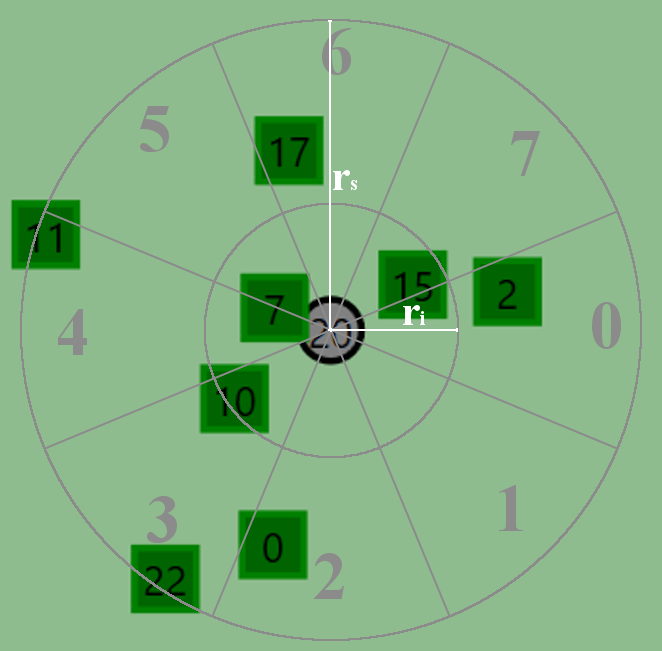
\includegraphics[scale=0.4]{Chapters/vision}
\end{figure}

Niech:
\begin{itemize}
    \item $r_{i}$ oznacza zasięg interakcji
    \item
     $L(a,b)= 
    \begin{cases}
        1,& \text{gdy } a\leq b\\
        0,              & \text{w p. p.}
    \end{cases}
    $
    \item $P_{k,0}...P_{k,n_{k}}$ reprezentuje wszystkie rośliny w zasięgu wzroku ($r_{s}$) w kierunku $k$, $k=0...7$. 
    \item $M(P)$ oznacza masę danej rośliny $P$
    \item $D(P)$ oznacza odległość rośliny $P$ od osiołka
    \item $C_{k} = \sum_{i=0}^{n_{k}} M(P_{k,i}) \cdot L(D(P_{k,i}),r_{i})  $
    \item $C = \sum_{d=0}^{7} C_{d}$
    \item $R'_{k} = \sum_{i=0}^{n_{k}} \frac{M(P_{k,i})}{D(P_{k,i}) - r_{i} + 1} \cdot (1-L(D(P_{k,i}),r_{i})) $
    \item $R_{k} = \frac{R'_{(k-1) \mod 8} + R'_{(k+1) \mod 8}}{2} + R'_{k}$
    \item $R = \sum_{d=0}^{7} R_{d}$
\end{itemize}
\clearpage
Wtedy:
\\$\textbf{CloseFoodDirections} = \sum_{d=0}^{7} 2^{d} \cdot L(\frac{C}{9},C_{d})$
\\$\textbf{FoodRichDirections} = \sum_{d=0}^{7} 2^{d} \cdot L(\frac{R}{9},R_{d})$

Tak więc bit \textbf{CloseFoodDirections} jest równy $1$, jeśli w wyznaczanym przez niego kierunku znajduje się więcej jedzenia w zasięgu interakcji niż przeciętnie. 

Bit \textbf{FoodRichDirections} jest równy $1$, jeśli w wyznaczanym przez niego kierunku, znajduje się poza zasięgiem interakcji (po przeskalowaniu względem odległości i uwzględnieniu kierunków sąsiednich) więcej jedzenia niż przeciętnie.

\section{Akcje}
Instrukcje, które kontroler może wydać osiołkowi są uproszczone, podobnie jak stany. Akcja w rozumieniu kontrolera składa się z dwóch elementów:
\begin{itemize}
    \item Rodzaj - pominięcie tury, ruch, jedzenie
    \item Kierunek - liczba od 0 do 7
\end{itemize}
Akcja taka jest jest po wybraniu tłumaczona na instrukcję w rozumieniu silnika symulacji. Próba zjedzenia obiera na cel najbliższą roślinę w danym kierunku, zaś ruch obiera kierunek odpowiadający zadanemu, dla uproszczenia odchylany w stronę najbliższej rośliny w tym kierunku.

\section{Parametry kontrolera}
Parametry kontrolera definiowane są w pliku .json z ustawieniami. Są to:
\begin{enumerate}
    \item\textbf{ProbabilityExponent} - zwiększa różnicę w prawdopodobieństwie między najlepszymi a najgorszymi akcjami
    \item\textbf{StartLearningRate} - początkowa wartość parametru $\alpha$, który wpływa na skalę zmian wprowadzanych do stanu kontrolera po każdej decyzji
    \item\textbf{LearningRateDamping} - zmniejsza wartość parametru $\alpha$ kontrolera z czasem poprzez mnożenie go przez tę liczbę w każdej turze
    \item\textbf{StartBaseActionScore} - początkowy \textbf{BaseActionScore}, który zapewnia niezerowe prawdopodobieństwo wszystkim możliwym akcjom
    \item\textbf{BaseActionScoreDamping} - zmniejsza faktyczny \textbf{BaseActionScore} kontrolera z czasem poprzez mnożenie go przez tę liczbę w każdej turze
    \item\textbf{Discount} - wartość parametru $\gamma$, który wpływa na balans między rozważaniem natychmiastowej nagrody płynącej z akcji i jej konsekwencji
\end{enumerate}

\section{Nauka}
Kontroler wykorzystuje prosty Q-Learning oparty o tabelkę definiującą funkcję $Q$, która każdej parze (stan,akcja) przyporządkowuje pewną wartość, która jest modyfikowana w czasie nauki. Na początku funkcja ta ma wartość 0 dla wszystkich argumentów.

Przyjmijmy, że w turze $t$ osiołek znajdował się w stanie $S_{t}$, jego \textbf{Hunger} wynosił $H_{t}$ i podjął akcję $A_{t}$. Doprowadziło go to do stanu $S_{t+1}$, w którym \textbf{Hunger} wynosi $H_{t+1}$. Niech $\Delta H = H_{t} - H_{t+1}$, $\alpha_{t} = \textbf{StartLearningRate} \cdot \textbf{LearningRateDamping}^{t}$ Wtedy:
\[Q_{t+1}(s_{t},a_{t})= Q_{t}(s_{t},a_{t}) \cdot (1-\alpha_{t}) + \alpha_{t} \cdot (\Delta H + \gamma \cdot max_{a}Q_{t}(s_{t+1},a))
\]

Dla wszystkich $(s,a)$ różnych od $(s_{t},a_{t})$ $Q_{t+1}(s,a) = Q_{t}(s,a)$

\section{Podejmowanie decyzji}
Po zaktualizowaniu funkcji $Q$ wybierana jest akcja do podjęcia w danej turze. Każda akcja ma pewne pradopodobieństwo zostania wybraną, zależne od wartości funkcji $Q$. Niech $\beta_{t} = \textbf{StartBaseActionScore} \cdot \textbf{BaseActionScoreDamping}^{t}$. Wtedy prawdopodobieństwo akcji $a$ w stanie $s_{t}$ wynosi:

$P_{t}(s_{t},a) = \frac{P'_{t}(s_{t},a)}{\sum_{a'}P'_{t}(s_{t},a')}$, gdzie

$P'_{t}(s_{t},a) = (Q_{t}(s_{t},a) - min_{a'}Q_{t}(s_{t},a') + \beta_{t})^{\textbf{ProbabilityExponent}}$

Parametr $\beta$ zapewnia niezerowe prawdopodobieństwo każdej możliwej akcji, dzięki czemu akcje uznane wcześnie za dobre nie dominują tych jeszcze niewypróbowanych. \textbf{ProbabilityExponent} zwiększa szanse wybrania dobrych akcji zmniejszając szanse wybrania złych.